%%%%%%%%%%%%%%%%%%%%%%%%%%%%%%%%%%%%%%%%%%%%%%%%%%%%
\documentclass[a4paper,fleqn,10pt,twocolumn]{SICE_ISCS}
%\usepackage{url}
\usepackage{ascmac}
\usepackage{amssymb}
%\usepackage{amsmath}
%\usepackage{hyperref}
%\usepackage{lmodern}
\usepackage{breqn}
\usepackage{bm}
\usepackage{comment}
\usepackage{pdfpages}
%\usepackage{HERE}
%\usepackage[version=3]{mhchem}%%化学式
%\usepackage{siunitx}
\usepackage[utf8]{inputenc}
\newcommand{\Tabref}[1]{{Table~\ref{#1}}}
\newcommand{\Equref}[1]{式(\ref{#1})}
\newcommand{\Figref}[1]{{Fig.~\ref{#1}}}
\newcommand{\blue}[1]{\textcolor{blue}{#1}} 
\title{Bonsensus Control for Resilient Multi-Agent Systems\\
	 Considering Leader Failure}

\author{Takuya Murakami${}^{1\dagger}$ and Toru Namerikawa${}^{2}$}
% The dagger symbol indicates the presenter.
\speaker{Takuya Murakami}

\affils{${}^{1}$School of Integrated Design Engineering, Keio University, Kanagawa, Japan\\
	    ${}^{2}$Department of System Design Engineering, Keio University, Kanagawa, Japan\\
(Tel: +81-45-563-1151; E-mail: muratakmit@keio.jp, namerikawa@sd.keio.ac.jp)\\
}
\abstract{%
In this paper, we study a consensus control problem for resilient multi-agent systems considering leader failure. We present cooperative control to solve the formation problem, enabling the agents to maintain relative positions even if any agent, including the leader, malfunctions. To accomplish this goal, we designed an algorithm that implements distributed observers for fault detection to assess each agent's reliability. The algorithm reduces the effect of faults by limiting information exchange with low-reliability agents.
Next, we extended the adjacency matrix so that any follower can replace the leader in response to the leader's failure.
Finally, we verify the proposed method through simulations.}

\keywords{%
Multi-Agent systems, Resilient systems, Fault detection, Formation.
}

\begin{document}

\maketitle

%-----------------------------------------------------------------------

\section{Introduction}
In recent years, mobile robots, including unmanned aerial vehicles (UAVs), have been widely used in various applications such as product delivery, information gathering, and search and rescue. In this context, the control of multi-agent systems, where multiple autonomous robots cooperate to enhance overall performance, has attracted significant attention and is actively studied. However, as the number of robots in these systems increases, the likelihood of malfunctions in some robots also grows. Despite this, relatively little research has focused on robot failures in multi-agent control methods.

Research on addressing failures in multi-agent systems has primarily focused on designing robust controllers to minimize the impact of failures on the overall system\cite{Davoodi,2017FTC,2018FTC}.However, such studies mainly deal with  failures that can be compensated for within the system. When failures exceed the compensation range, their impact can propagate and disrupt the entire system.

Consensus and formation are also typical problems in the control of multi-agent systems. This is because achieving convergence of state variables, such as velocity and position to the same value is often useful. The leader-follower structure is frequently employed for effective control. Research addressing agent failures in leader-follower structures\cite{Resi_leaderfollower} does not consider leader failure. Moreover, research considering leader replacement\cite{Affection} poses a high risk of deadlock when a follower failure occurs.

In this study, we focus on two aspects of formation control for multi-agent systems with a leader-follower structure: resilient control that can address failures difficult to compensate for, and control designed to handle leader failures.

Specifically, we aim for a multi-agent system with a leader-follower structure that can maintain formation even when a failure occurs in any agent, including the leader. Based on the reliability level of each agent, the system minimizes the impact of the failed agent by limiting the information exchange with the faulty agent. In addition, we propose a system that allows the leader to be changed at any time in the event of a leader agent failure.

This paper is organized as follows. Chapter 2 introduces the model used in this study, including formation control through a consensus algorithm and the representation of failure. Chapter 3 presents algorithms for fault detection, strategies to block the influence of faulty agents, and methods for enabling leader replacement. Finally, Chapter 4 verifies the effectiveness of the proposed method through numerical simulations.

In this paper, the subscripts $i$ and $j$ denote the $i$-th and $j$-th agents, respectively.

\section{Problem Settings}
An overview of the problem settings in this study is presented in \Figref{Nice_image_fault}.
The objective is to maintain the formation of a group of mobile robots that consists of one leader and $N-1$ followers, for a total of $N$ robots, even in the presence of failures among agents, including the leader, while ensuring that the non-faulty agents can sustain the formation.
\begin{figure}[b]
	\begin{center}
		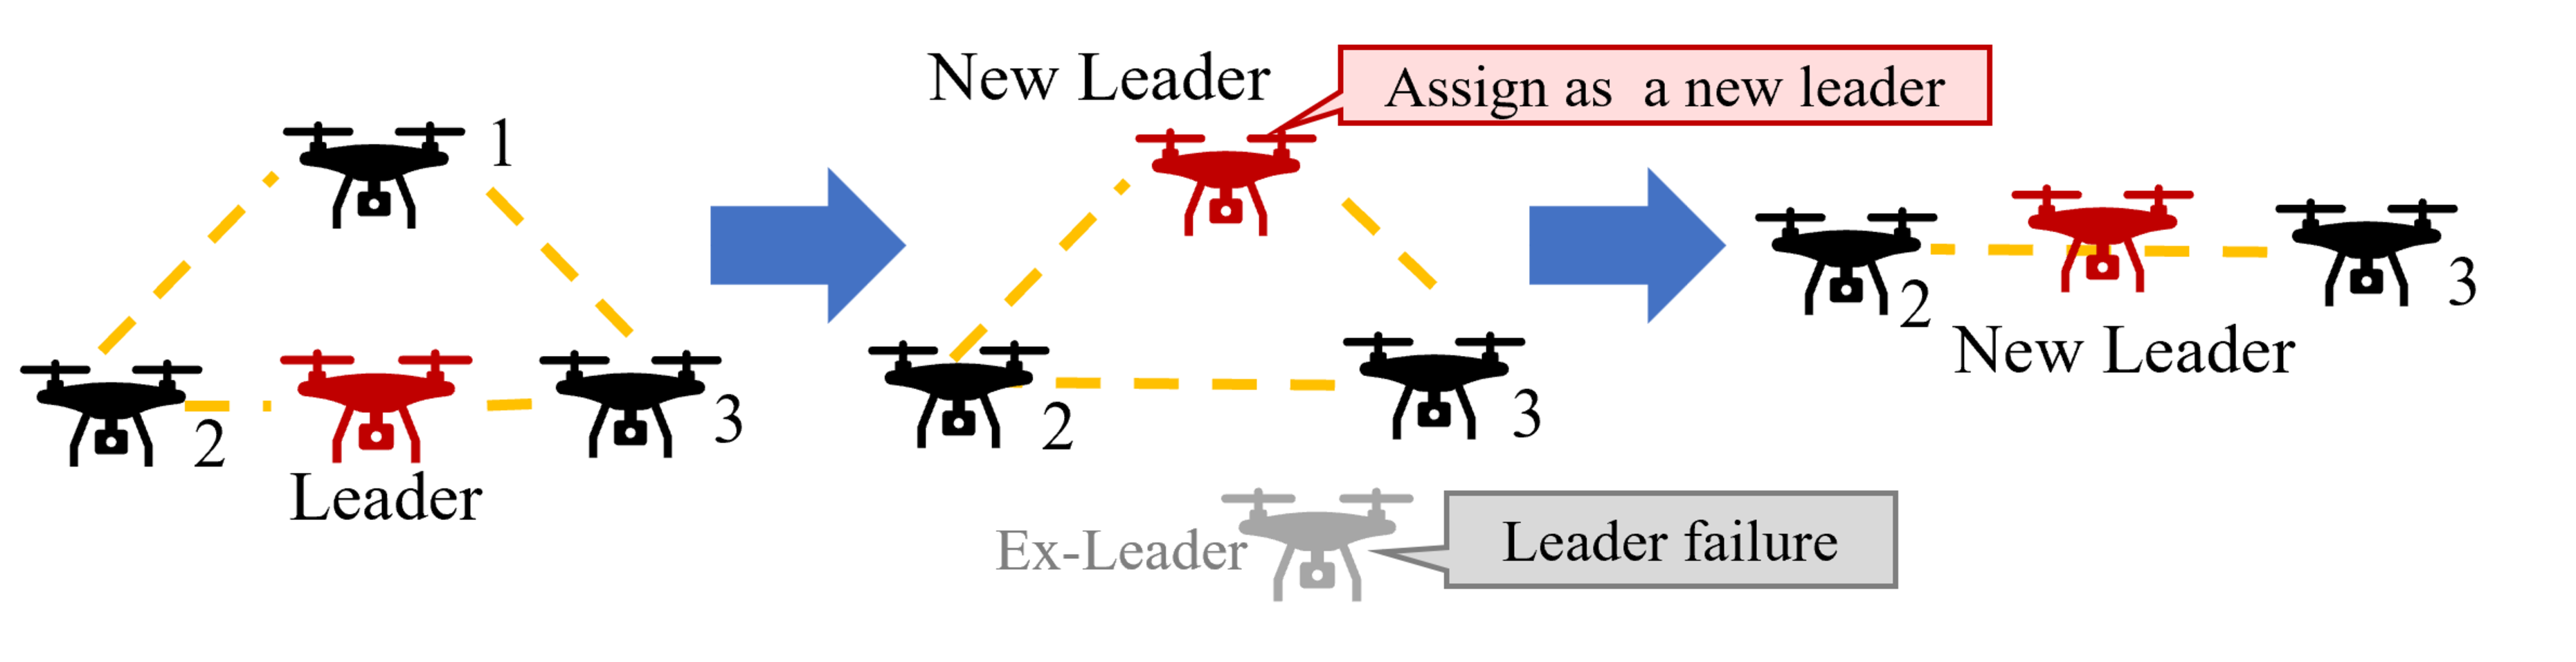
\includegraphics[width=\linewidth]{Fig/Nice_image_fault.eps}
		\caption{Image of problem settings.}
		\label{Nice_image_fault}
	\end{center}
	\vspace{-2mm}
\end{figure}

\subsection{Modeling a Multi-Agent System}
This research focuses on a model consisting of a system of $N$ identical agents, each with the same altitude $z_i$, with a primary focus on motion within a 2D plane. The model is described by the following equation:

\begin{equation}
	\label{modeling}
	\dot{r}_i=u_i,\ \ \ \ \ (i=1,2,...N),
\end{equation}

\noindent where $r_i \in {\mathbb{R}}^2$ and $u_i \in {\mathbb{R}}^2$ are the position and the control input of agent $i$, respectively. We use graph theory to describe the network structure of $N$ agents in a multi-agent system. A graph $ {\mathcal{G}} = (\mathcal{V}, \mathcal{E})$ is used to describe the information flow among agents. The vertex set ${\mathcal{V}} =\{v_1, v_2, \ldots, v_N\}$ consists of the vertices $v_i$, and the edge set ${{\mathcal{E}}\in {\mathcal{V}}\times{\mathcal{V}}}$ represents the edges of the graph. The edge $(v_i,v_j)$ indicates the presence of a network path from agent $i$ to agent $j$.

A graph in which all edges are bidirectional is called an undirected graph; if the edges are not bidirectional, the graphs are called a directed graph. In this paper, we focus on directed graphs.

To algebraically represent a graph, the adjacency matrix $\mathcal{A}$, the degree matrix $\mathcal{D}$, and the graph Laplacian $\mathcal{L}$ are used. The elements of the adjacency matrix ${\mathcal{A}} = [a_{ij}]$ are defined as follows:

\begin{equation}
	a_{ij}=
	\begin{cases}
		1 &\ \ {\mathrm{for}}\ i\ \mathrm{connected\ from}\ j\\
		0 &	\ \mathrm{otherwise}
	\end{cases}.
\end{equation}

In a multi-agent system, this means that if the $i$-th agent receives information from the $j$-th agent, the corresponding $a_{ij}$ is set to 1, and 0 otherwise.

The degree matrix $\mathcal{D}$ is diagonal matrix given by \begin{equation} {\mathcal{D}} = {\mathrm{diag}}(deg(v_1), deg(v_2), \dots, deg(v_N)), \end{equation}
where $deg(v_i)$ represents the number of communication links connect to node $v_i$.
\subsection{Formation Control with Consensus Algorithm}
We explain the control methods for achieving formation among multiple mobile robots.

We employ a method that applies consensus algorithms to formation control to achieve the formation{\cite{栗城モデル}}. In this method, the followers track the leader's movements while maintaining the formation shape, operating under a leader-follower structure. 
Next, we make the following assumption.\\
\textbf{Assumption 1} Every follower must be connected to the leader.

The control input for agent $i$ in a system consisting of $N$ agents, where there is one leader and $N-1$ followers, is given by

\begin{small}
\begin{align}
	\label{kuriki_consensus}
	\dot{r}_i=&\frac{1}{\sum_{j=1}^{N}a_{ij}}
	\bigg\{\sum_{j=1}^{N}a_{ij}\big(-k(h_i - h_j)+\dot{r}_j+(\dot{d}_i-\dot{d}_j)\big)\bigg\}.
	%\bigg\{\sum_{j=1}^{N}a_{ij}\big(-k(h_i - h_j)\big)\bigg\} \notag\\
	%&+\frac{1}{\sum_{j=1}^{N}a_{ij}}
	%\bigg\{\sum_{j=1}^{N}a_{ij}\big(\dot{r}_j+(\dot{d}_i-\dot{d}_j)\big)\bigg\}.
\end{align}
\end{small}

\noindent where $h_i \in {\mathbb{R}}^2$ is the time-varying vector, defined as the difference between the position of follower $r_i$, and the target relative position $d_i \in {\mathbb{R}}^2$ measured from the leader. The meaning of each symbol is illustrated in \Figref{DefinitionofSymbols(L-F)}. The leader assigns the target relative position $d_i$ for all agents with respect to leader's own position $r_L$ and broadcasts this information to the directly connected followers based on the network structure. Through this, the leader transmits the target relative position of each agent while moving, and each follower determines its control input based on the states of adjacent followers and aims to reach consensus on the target relative position by aligning each $h_i$ with $r_L$ at the end. 

\begin{figure}[b]
	\begin{center}
		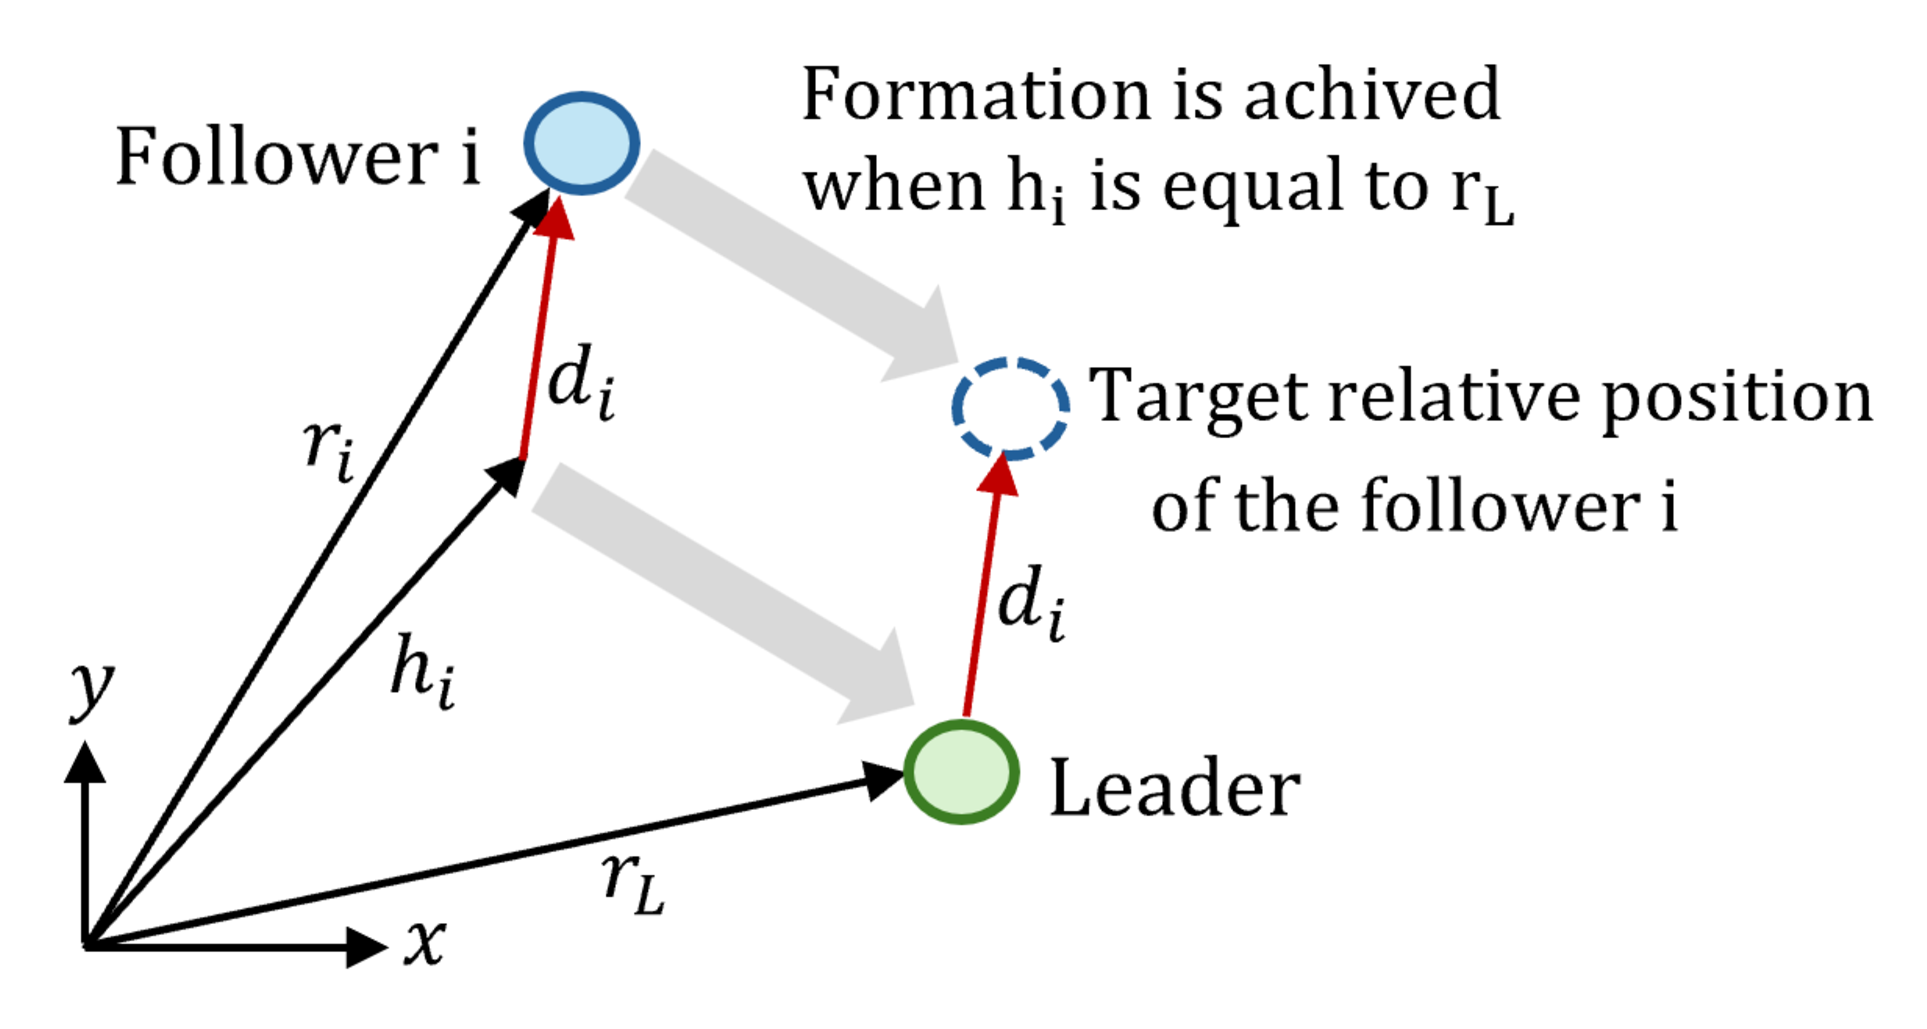
\includegraphics[width=75mm]{Fig/DefSymbol_(L-F).eps}
		\caption{Definition of symbols: Follower $i$ and leader.}
		\label{DefinitionofSymbols(L-F)}
	\end{center}
	\vspace{-1mm}
\end{figure}

\begin{figure}[b]
	\begin{center}
		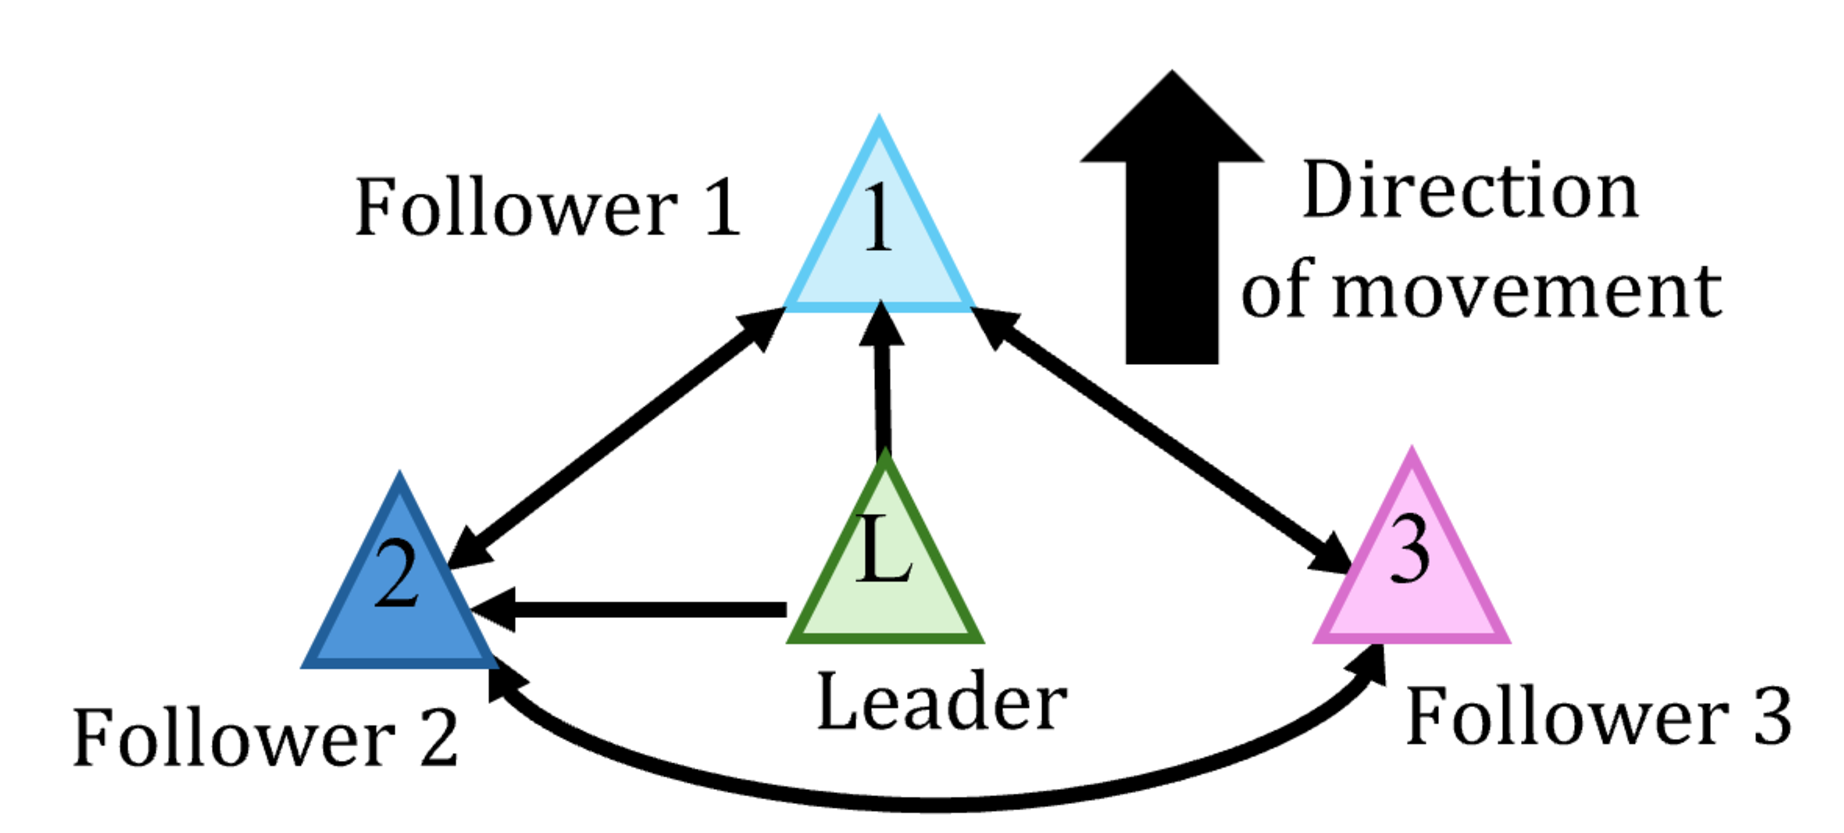
\includegraphics[clip,width=73mm]{Fig/Topology.eps}
		\caption{Target shape of formation and topology.}
		\label{Topology}
	\end{center}
	%\vspace{-1mm}
\end{figure}

The target formation is designed such that the followers surround the leader, as shown in \Figref{Topology}. We now present an example where the formation is successfully achieved. The initial position of the leader is set at origin (0,0), and the leader moves counterclockwise along a half-ellipse with a major axis of 12 meters and a minor axis of 10 meters.

The trajectories of all agents are shown in \Figref{Trajectorysample}, with circles and squares representing the starting and goal points, respectively. The followers  move in a formation around the leader as it moves. \Figref{Errorsample} illustrates the deviation of each agent from the target relative position with respect to the leader. All agents reach their target relative positions, and the formation is remains stable.



\begin{figure}[t]
	\begin{center}
		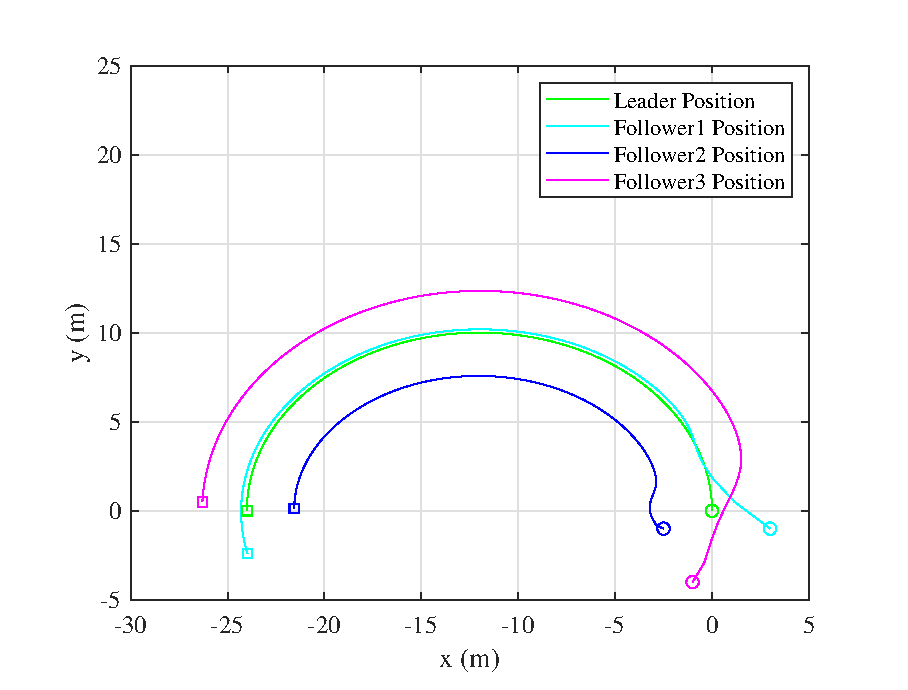
\includegraphics[clip,width=\linewidth]{Fig/sampletrajectry.eps}
		\caption{Trajectory of all agents.}
		\label{Trajectorysample}
	\end{center}
	\vspace{-2mm}
\end{figure}


\begin{figure}[t]
	\begin{center}
		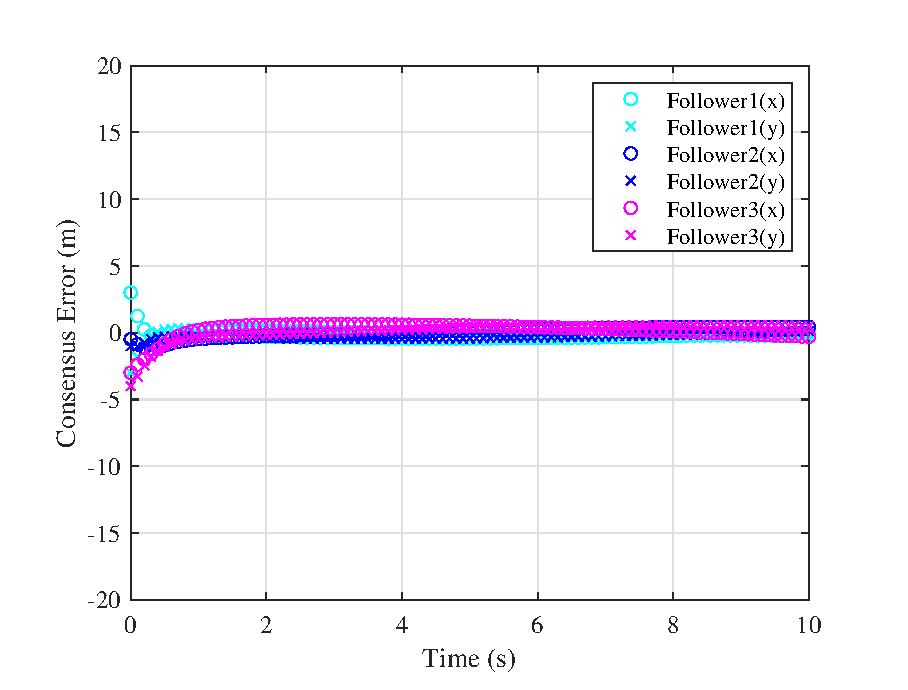
\includegraphics[clip,width=\linewidth]{Fig/sampleconsensus.eps}
		\caption{Consensus errors from the target relative positions from the leader.}
		\label{Errorsample}
	\end{center}
	\vspace{-4mm}
\end{figure}

\subsection{Assumed Failure in this research}
We explain the failures assumed in this study. Various types of failures can be considered in mobile robots, but this paper focuses on actuator failures, where control inputs are replaced by incorrect values. Actuator failures are classified into the following four types \cite{4types_fault}:
(a) Hard-over (fixed at maximum input value), 
(b) Loss of effectiveness (a certain percentage of the command value is reduced), 
(c) Lock in place (fixed at the input value at the time of failure), and 
(d) Float (input fixed at zero). 

To focus on responses that are difficult to compensate for, this study highlights (a) Hard-over.

Hard-over can be expressed by
\begin{align}
	u_i = f_{max},
\end{align}
\noindent where $f_{max} \in {\mathbb{R}}^2$ represents the maximum input value in the system, which becomes constant after the failure occurs. Next, we make an assumption as follows:\\
\textbf{Assumption 2} There are no observation errors such as sensor information for each agent, and the failed agent continues to exchange information with adjacent agents just like the non-faulty agents.

Under this assumption, it is necessary to detect the occurrence of failures in a distributed manner based on the behavior of the faulty agent and to implement control methods that block the influence of the agent.


\section{Resilient Design Considering Failure}
We present the fault detection algorithm, control strategies to reduce the impact of failed agents, and  methods for leader replacement.
The design of the distributed observer utilized for fault detection is described. Using equation (\ref{kuriki_consensus}) as a basis, the distributed observer is constructed as follows:

\begin{small}
\begin{align}
	\dot{\hat{r}}_i=&\frac{1}{\sum_{j=1}^{N}a_{ij}}
	\bigg\{\sum_{j=1}^{N}a_{ij}\big(-k(\hat{h}_i - \hat{h}_j)\big)\bigg\} \notag\\
	+&	\frac{1}{\sum_{j=1}^{N}a_{ij}}
	\bigg\{\sum_{j=1}^{N}a_{ij}\big(\dot{\hat{r}}_j+(\dot{d}_i-\dot{d}_j)\big)\bigg\} +m\epsilon_i,
\end{align}
\end{small}

\noindent where $\hat{h}_i\in{\mathbb{R}}^2$ and $\hat{r}_i\in{\mathbb{R}}^2$ are the estimated values of $h_i$ and $r_i$.
The residual $\epsilon_i\in{\mathbb{R}}^2$ is expressed as the sum of the difference between the agent's own observed and estimated values, and the difference between the observed and estimated values of the agents adjacent to $i$, is shown in

\begin{align}
	\epsilon_i =\{r_i-\hat{r}_i\}+\sum_{j=1}^{N}a_{ij}\{r_j-\hat{r}_j\}.	
	\vspace{-3mm}
\end{align}

Therefore, distributed observers adapted for formation control and the residual $\epsilon_i$, which is used for feedback to the observers, can be obtained.
Fault detection can be achieved by combining the residual $\epsilon_i$ with a predefined threshold. 
However, under real conditions, it is assumed that agents recover from temporary failures and short-term disturbances, such as sudden gusts. Therefore, it is not appropriate to immediately cut off connections with a faulty agent solely based on fault detection. Considering this, we design algorithms that adjust the reliability of each agent, and the weights of connections between agents are determined based on this reliability.
The calculation methods for the reliability of each agent are described as follows.

With reference to \cite{Affection}, we design a reliability measure for evaluating the trustworthiness of each agent. Each agent detects failures when the residual exceeds the threshold, as indicated by $\|\epsilon_i\|>\tau$. Each agent increases its level of  ``disappointment'' based on the duration of the detected failure. The ``disappointment'' is expressed by

\begin{align}	
	\dot{\delta_i}=\delta_i(e^{-\alpha}-1)+\rho_i(1-e^{-\beta t_i})\\
	\rho_{i}=
	\begin{cases}
		1 &\ \ \|\epsilon_i\|> \tau \\
		0 &	\ \mathrm{otherwise}
	\end{cases}.
\end{align}

\noindent where $\alpha\in\mathbb{R}$ and $\beta\in\mathbb{R}$ are positive parameters used to adjust the rates of decay and increase, respectively, and $t_i\in\mathbb{R}$ represents the duration for which agent $i$ detects a failure. When a failure is detected in agent $i$, $\rho_i$ is 1, and 0 otherwise. While agent $i$ continues to detect a failure, the second term increases, which causes $\delta_i\in\mathbb{R}$ to increase. When the agent recovers from the failure, the first term causes $\delta_i$ to decrease.

Additionally, by determining the reliability \(\gamma_i \in \mathbb{R}\) is represented by 
\begin{equation}
	\gamma_i=\min(1-\delta_i,1).
\end{equation}	
It becomes possible to express the reliability within the range from 0 to 1.

Next, to represent the reliability of each agent, we introduce a diagonal matrix \({\mathcal{T}} \in {\mathbb{R}}^{N \times N}\), which is expressed as 
\begin{equation}
	{\mathcal{T}}={\mathrm{diag}}(\gamma_1,\gamma_2,......\gamma_N).
\end{equation}
Then, by multiplying \(\mathcal{T}\) with the initial adjacency matrix \({\mathcal{A}}_0 \in {\mathbb{R}}^{N \times N}\), which is represented by
\begin{align}
	{\mathcal{A}}_0=
	\begin{bmatrix}
		0 & a_{12} & ... & a_{1N}\\
		a_{21} & 0 & ... & a_{2N}\\
		\vdots & \vdots & \ddots & \vdots\\
		a_{N1} & a_{N2} & ... & 0\\ 
	\end{bmatrix}.
\end{align}
Time varying adjacency matrix \({\mathcal{A}} \in {\mathbb{R}}^{N \times N}\) is obtained by
\begin{align}
	{\mathcal{A}}	= {\mathcal{A}}_0 {\mathcal{T}} =
	\begin{bmatrix}
		0 & a_{12}\gamma_2 & ... & a_{1N}\gamma_{N}\\
		a_{21}\gamma_1 & 0 & ... & a_{2N}\gamma_{N}\\
		\vdots & \vdots & \ddots & \vdots\\
		a_{N1}\gamma_1 & a_{N2}\gamma_2 &... & 0\\ 
	\end{bmatrix}.
\end{align}

The network connection can be reconstructed to mitigate the influence of faulty agents by changing \({\mathcal{A}}\) according to the reliability of each agent.

\subsection{Extension of the adjacency matrix}
Assuming the replacement of the leader, we consider an algorithm that controls both the leader and the followers using the same control law, allowing for alternation between them.


First, based on the initial adjacency matrix \({\mathcal{A}}_0\), we express \({{\mathcal{B}}}_0 \in {{\mathbb{R}}}^{(N+1) \times (N+1)}\) by adding target position information from the base station or another group, resulting in \(N+1\) rows and \(N+1\) columns as follows:

\begin{align}
	{\mathcal{B}}_0=
	\begin{bmatrix}
		0     & a_{12} & ... & a_{1N} & 0\\
		a_{21}& 0 & ... & a_{2N} & 0\\
		\vdots& \vdots & \ddots &\vdots& \vdots\\
		a_{N1}& a_{N2}&...&... & \vdots\\
		0 & 0 & ... &...& 0\\ 
	\end{bmatrix}.
\end{align}
Next, to change the control inputs for the leader and followers according to the replacement of the leader, we introduce the leader flag \(l_i\), which is expressed by

\begin{align}
	l_i=
	\begin{cases}
		0 &\ \ \  {\mathrm{for}}\ i\ \mathrm{is\ a\ leader}\\
		1 &\ \ \  \mathrm{otherwise}
	\end{cases}.
\end{align}
Then, using the leader flag \(l_i\), we design the system so that the target position is communicated to the leader while blocking information from the followers to the leader. First, we express the diagonal matrix \({\mathcal{C}} \in {\mathbb{R}}^{(N+1) \times (N+1)}\) and the matrix \({\mathcal{E}} \in {\mathbb{R}}^{(N+1) \times (N+1)}\) which are described by
\begin{equation}
	{\mathcal{C}}={\mathrm{diag}}(l_1,l_2,...l_{N},1),
	\vspace{-2mm}
\end{equation}

\begin{align}
	\mathcal{E}=
	\begin{bmatrix}
		0     & 0      & ...    & 0    & 1-l_1\\
		0     & 0      & ...    & 0    & 1-l_2\\
		\vdots& \vdots & \ddots &\vdots& \vdots\\
		0     & 0      & ...    &0     & 1-l_N\\
		0     & 0      & ...    &0     & 0\\ 
	\end{bmatrix}.
	\vspace{-2mm}
\end{align}

Then, the target position is communicated to the leader while blocking information from the followers to the leader.

\begin{equation}
	{\mathcal{B}}_1={\mathcal{C}}{\mathcal{B}}_0+{\mathcal{E}}.
\end{equation}
By installing ${\mathcal{B}}_1$, the leader can block information from the followers because all elements in the leader's row are set to 0, while ensuring that the target position information is communicated only to the leader because only the \(N+1\) column is set to 1.


Next, to control each agent, the extended adjacency matrix \(\mathcal{B}\) is obtained by multiplying the reliability matrix \(\mathcal{T}\) with \({\mathcal{B}}_1\), which is represented as: 
\begin{equation}
	{\mathcal{B}}={\mathcal{B}}_1\mathcal{T}.
\end{equation}

Then, we describe the conditions for leader replacement. Initially, agent \(N\) is the leader; however, when the reliability of the leader \(\gamma_N = 0\), the process of re-electing a leader begins. The new leader is selected as the agent \(i\) with the smallest number among the agents adjacent to the current leader. In the previous steps, we implemented steps to mitigate the influence of low-reliability agents and extended the adjacency matrix to allow for leader replacement in response to leader failures. 

\subsection{Consensus algorithm considering both the leader and the followers}
Next, we explain a consensus algorithm that considers both the leader and the followers. To ensure that the leader agrees on the target position, we modify equation (\ref{kuriki_consensus}) as follows:
\begin{small}
\begin{align}
	\dot{r}_i & =\frac{1}{\sum_{j=1}^{N+1}a_{ij}}
	\bigg\{\sum_{j=1}^{N+1}a_{ij}\Big(-k(r_i - r_j)+\dot{r}_j\Big)\Big)\bigg\}\notag\\
	& +l_i\frac{1}{\sum_{j=1}^{N+1}a_{ij}}
	\bigg\{\sum_{j=1}^{N+1}a_{ij}\Big(k(d_i-d_j)+(\dot{d}_i-\dot{d}_j)\Big)\bigg\}.	
\end{align}
\end{small}
This equation allows the followers to use a control law that is the same as (\ref{kuriki_consensus}), while the leader sets all terms related to the target relative positions \(d_i\) and \(d_j\) to zero, therebyenabling the leader to reach consensus on the target position indicated by the base station or similar equipment.

\section{Simulations}
In this section, numerical simulations are conducted to verify the effectiveness of the proposed control methods. The simulation conditions are described below. The desired formation shape, including the leader's movement trajectory, is similar to that shown in \(\text{Fig.} \ref{Topology}\), and a hard-over failure occurs in the leader agent when \(t \geq 3\). Comparisons are made between the cases with and without the proposed control method.

The simulation parameters are shown in Table \(\ref{parameter_ADLSM}\).



\begin{table}[b]
	\begin{center}
		\caption{Parameter of simulation}
		\label{parameter_ADLSM}
		\begin{tabular}{c c c} \hline
			Symbol & Parameter & Value \\ \hline
			$k$ & Control gain & 5\\
			$\tau$ & Threshold of fault detection & 0.7\\
			$\alpha$ & Recoverability of trust & 0.1\\
			$\beta$ & Sensitivity of fault & 0.1\\ 
			$m$ & Distributed observer gain  & 5\\
			$f_{max}$ & Hard-over signal (Maximum Input) & [-3 3]\\ \hline
		\end{tabular}
	\end{center}
	\vspace{-1mm}
\end{table}

We demonstrate the simulation results as follows. The trajectories of each agent are shown in \(\text{Fig.} \ref{HC_L_T}\), the residuals of the estimated and observed values are displayed in \(\text{Fig.} \ref{HC_L_R}\), and the deviations from the target positions are illustrated in \(\text{Fig.} \ref{HC_L_E}\). In each of these figures, the results on the left correspond to the scenario without the proposed control law, while the results on the right reflect the scenario with the proposed control law. 

\(\text{Fig.} \ref{HC_L_T}\) shows that, after the leader's failure, follower 1 takes over the target position as the new leader, while the other followers maintain the formation without being affected by the failed agent. 

In \(\text{Fig.} \ref{HC_L_R}\), it is observed that not only do the residuals of the faulty agent increase, but also the residuals of the non-faulty agents. However, when the proposed control law is applied, the residuals of the non-faulty agents converge again after the failure occurs. 

Furthermore, \(\text{Fig.} \ref{HC_L_E}\) shows that all non-faulty agents remain at the target position. These results indicate that is possible to maintain the formation even after a fault occurs in the leader, which is difficult to compensate for, by replacing the leader.


\begin{figure}[b]
	\begin{center}
		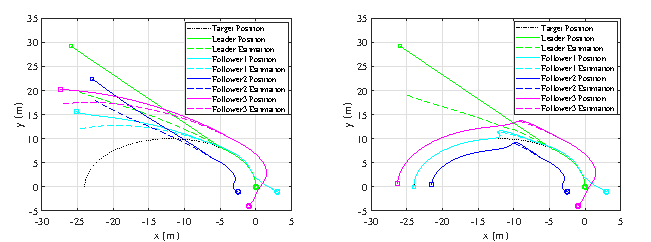
\includegraphics[clip,width=84mm]{Fig/Leader_Trajectory_2ko1.eps}
		\caption{Comparison of the trajectory of leader failure. (left: conventional, right: proposed.)}
		\label{HC_L_T}
	\end{center}
	\vspace{-2mm}
\end{figure}

\begin{figure}[b]
	\begin{center}
		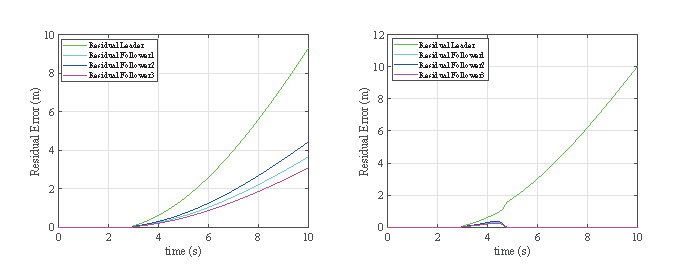
\includegraphics[clip,width=84mm]{Fig/Leader_Residual_2ko1.eps}
		\caption{Comparison of the residual errors of leader failure. (left: conventional, right: proposed.)}
		\label{HC_L_R}
	\end{center}
	\vspace{-2mm}
\end{figure}

\begin{figure}[b]
	\begin{center}
		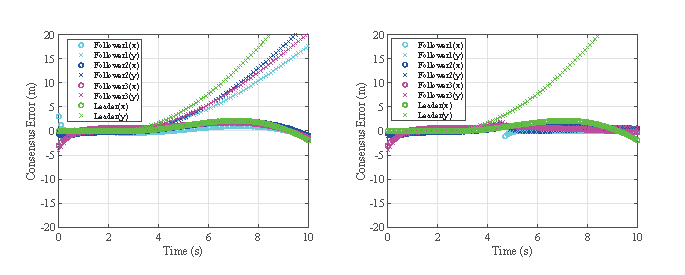
\includegraphics[clip,width=84mm]{Fig/Leader_Consensus_2ko1.eps}
		\caption{Comparison of the consensus errors of leader failure. (left: conventional, right: proposed.)}
		\label{HC_L_E}
	\end{center}
	\vspace{-3mm}
\end{figure}

\section{Conclusions and Future Work}
In this study, we focused on achieving formation control for multi-agent systems considering leader failures. We utilized a leader-follower structure in multi-agent systems, employing distributed observers for each agent to assess their reliability based on fault detection results. By blocking information exchange with faulty agents according to their reliability, we implemented a system to minimize the impact of failed agents. Additionally, we constructed a system that allows for leader replacement in the event of a fault, confirming through numerical simulations that formation can still be achieved even when an agent, including the leader,  malfunctions.

Future challenges include theoretical discussions of fault detection and related topics. While various parameters were determined experimentally in this study, we aim to further explore the theoretical aspects, including convergence.


%%%%%%%%%%%%%%%%% BIBLIOGRAPHY IN THE LaTeX file !!!!! %%%%%%%%%%%%%%%%%%%%%%
\begin{thebibliography}{9}
\bibitem{Davoodi}M.R. Davoodi, N. Meskin, and K. Khorasani, ``Simultaneous fault detection and control design for a network of multi-agent systems'' {\it Automatica}, Vol. 66, pp. 185-194, 2016.

\bibitem{2017FTC} P. Yang, B. Ma, Y. Dong and J. Liu, ``Adjustable Parameter-Based Distributed Fault Estimation Observer Design for Multiagent Systems With Directed Graphs,'' {\it IEEE Transactions on Cybernetics}, Vol. 47, No. 2, pp. 306-314, 2017.

\bibitem{2018FTC} K. Zhang, B. Jiang and P. Si, ``Fault-tolerant Consensus of Leader-following Multi-agent Systems Based on Distributed Fault Estimation Observer,'' {\it International Journal of Control, Automation and Systems}, Vol. 16, No. 5, pp. 2354-2362, 2018.

\bibitem{Resi_leaderfollower}H. Rezaee, T. Parisini and M. M. Polycarpou, `` Resiliency in dynamic leader-follower multiagent systems,'' {\it Automatica}, Vol. 125, 109384, 2021.     

\bibitem{Affection}F. Li, T. Ding, M. Zhou, K. Hao and L. Chen, ``An Affection-Based Dynamic Leader Selection Model for Formation Control in Multirobot Systems,'' {\it IEEE Transactions on Systems, Man, and Cybernetics: Systems}, Vol. 47, No. 7, pp. 1217-1228, 2017.

\bibitem{栗城モデル}Y. Kuriki and T. Namerikawa, ``Formation Control of UAVs with a Fourth-Order Flight Dynamics,'' {\it SICE Jounal of Control, Measurement and System Integration}, Vol. 7, No. 2, pp. 74-81, 2014.

\bibitem{4types_fault}J. Boskovic and R. K. Mehra, ``Failure Detection, Identification and  Reconfiguration in Flight Control,'' {\it Fault Diagnosis and Fault Tolerance for Mechatronic Systems: Recent Advances}, Chapter 1, pp. 129-167, Springer, 2003.

\end{thebibliography}

\end{document}

